% THIS IS SIGPROC-SP.TEX - VERSION 3.1
% WORKS WITH V3.2SP OF ACM_PROC_ARTICLE-SP.CLS
% APRIL 2009
%
% It is an example file showing how to use the 'acm_proc_article-sp.cls' V3.2SP
% LaTeX2e document class file for Conference Proceedings submissions.
% ----------------------------------------------------------------------------------------------------------------
% This .tex file (and associated .cls V3.2SP) *DOES NOT* produce:
%       1) The Permission Statement
%       2) The Conference (location) Info information
%       3) The Copyright Line with ACM data
%       4) Page numbering
% ---------------------------------------------------------------------------------------------------------------
% It is an example which *does* use the .bib file (from which the .bbl file
% is produced).
% REMEMBER HOWEVER: After having produced the .bbl file,
% and prior to final submission,
% you need to 'insert'  your .bbl file into your source .tex file so as to provide
% ONE 'self-contained' source file.
%
% Questions regarding SIGS should be sent to
% Adrienne Griscti ---> griscti@acm.org
%
% Questions/suggestions regarding the guidelines, .tex and .cls files, etc. to
% Gerald Murray ---> murray@hq.acm.org
%
% For tracking purposes - this is V3.1SP - APRIL 2009

\documentclass{acm_proc_article-sp}

\usepackage{hyperref}
\usepackage{subfig}

\begin{document}

\title{Camera Interact: An Educational Introduction to Cameras}

\numberofauthors{2}
\author{
\alignauthor
Sam Lau\\
       \affaddr{UC Berkeley}\\
       \affaddr{EECS}\\
       \email{samlau95@berkeley.edu}
\alignauthor
Jeronimo Mora\\
       \affaddr{UC Berkeley}\\
       \affaddr{Mechanical Engineering}\\
       \email{jeronimomora@berkeley.edu}
}

\date{5 May 2017}


\maketitle
\begin{abstract}
Camera Interact is an educational project to explain how cameras work. We take a ground-up approach to explanation, starting from basic sensor and light behavior and building up to a complete camera model. Instead of traditional text and image-based approaches, we emphasize animation and user interaction as teaching tools. A demo is created for the user to experiment with.
\end{abstract}

\keywords{CS284, Computer Graphics, Cameras, three.js, WebGL} % NOT required for Proceedings

\section{Introduction}
Cameras have a lot of moving parts, literally and figuratively. For someone
trying to understand how cameras work, the number of new vocabulary terms they
encounter (f-stop, aperture, shutter speed, FOV, circle of confusion etc.)
would alone be discouraging. Unfortunately, previously available work often
explained the usage of camera parameters without giving intuition, leading
students towards rote memorization instead of actual understanding
\cite{robertsinteract}. Existing applets for explaining cameras typically only
focus on one narrow parameter of the camera at a time \cite{stanfordinteract},
helping students understand that particular concept but making it difficult to
connect ideas together.

We assume that our user previously knows that:

\begin{enumerate}
  \item Rays of light travel in straight lines.
  \item Light takes on color.
\end{enumerate}

With these basic assumptions, we take a ground-up approach to explaining
how and why cameras work. By using animations that also allow the user to
interactively examine the scene we can help the user build intuition and
understanding.

We explain the following topics in our project:

\begin{enumerate}
  \item Pinhole cameras
  \item Field of view
  \item Aperture and depth of field
\end{enumerate}

Each of these topics has its own challenges when an individual is learning
about cameras for the first time. We identify some of the major challenges for
each of these topics and discuss our approach to helping the learner develop
a understanding.

\subsection{Pinhole Cameras}

Pinhole cameras are one of the simplest tools of creating and recording an
image.

\begin{figure}[h]
\caption{Diagram of pinhole camera \cite{pinhole}}
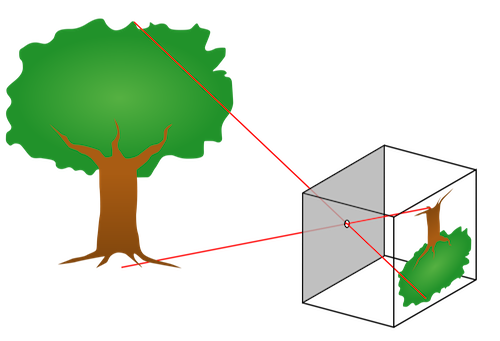
\includegraphics[width=8cm]{images/pinhole.png}
\end{figure}

In the pinhole camera, a small aperture allows a clear image to form on the
image plane. Learners typically have difficulty understanding:

\begin{enumerate}
  \item Why the aperture needs to be small to allow a clear image to form.
  \item Why the image formed is upside-down.
\end{enumerate}

We attempt to address these questions in our project by showing empirically
that the resulting will be completely blurred out if the aperture is too large.
Then, by drawing the light rays as they pass through the pinhole, the user can
immediately see why the resulting image is upside-down.

\subsection{Field of view}

Field of view refers to how much of the scene is captured on the resulting
image. In the context of cameras, field of view is typically modified by the
sensor size ($ h $) and the focal length ($ f $) according to the following
formula:

\[ \text{FOV} = 2 \arctan \left(\frac{h}{2f}\right) \]

However, from this equation alone it is unclear intuitively why:

\begin{enumerate}
  \item Increasing the sensor size increases the field of view.
  \item Increasing the focal length decreases the field of view.
\end{enumerate}

Using an interactive ray-tracing scene, we answer these questions by showing
that the field of view is determined by which rays of light reach the sensor.
We then show that both increasing the sensor size and decreasing the focal
length allow rays of light from wider angles to reach the sensor.

\subsection{Aperture and depth of field}

Lenses allow cameras to capture significantly more light than a pinhole camera
with a small aperture. In addition, they allow for depth of field adjustments
by changing the aperture size. The term circle of confusion is used to describe
how much an object is defocused on the image and is associated with the
following formula:

\[ C = A \frac{|z_s - z_i|}{z_i} \]

This topic typically raises the following questions:

\begin{enumerate}
  \item Why do lenses create a circle of confusion?
  \item Why does the circle of confusion increase as the aperture increases?
\end{enumerate}

We answer these questions in our project by showing how rays from an object
converge onto the image plane when the object is in focus. Then, we move the
object backward and show that the rays don't converge exactly, resulting in a
blurred image and thus the circle of confusion. We show empirically that the
circle of confusion decreases as we shrink the aperture through tracing rays
through the lens. Finally, we show that when the aperture is very small, as in
the case of the pinhole camera, the circle of confusion is also very small.

\section{Implementation}
\smallskip
\subsection{Interactive Camera Demo}
In order to create the interactive camera demo we made use of three.js
\cite{threejs}, a javascript package written over WebGL to create and render 3D
scenes in the browser. An image of the demo is provided in Fig. 2 below. We
create a scene consisting of a few objects and place a camera (the main camera)
overhead such that the entire scene can be seen. The view from this camera is
rendered into a window at the top of the given webpage. A second camera (the
static camera) is placed closer to the objects in the scene and has its view
rendered into a smaller window below the main camera's render window. The
purpose of the static camera is to render a "picture" of what a camera would
generate when using the parameters set by the user. The user has three
parameters to choose from: field of view (FOV), shutter speed, and fStop. When
the field of view parameter is changed, the field of view of the static camera
is changed as a result (lower field of view leads to a telephoto-like effect).
We also include two lines which are drawn in the main camera's scene emanating
from the location where the static camera is placed. As the FOV is changed,
these lines update to show the user how wide or narrow their current FOV is.
Changing either the shutter speed or the fStop will affect the scene lighting.
We created three functions that take input from the controls and update the
respective scene elements (the static camera's FOV and lighting will change and
the main camera's FOV lines will update). The functions are called within the
render loop so the effects can be seen in real-time.

\begin{figure}[h]
\caption{Interactive Camera Demo }
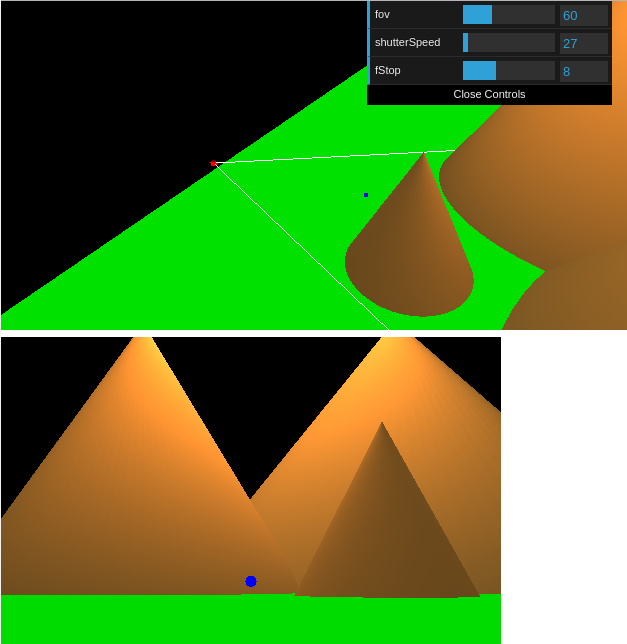
\includegraphics[width=8cm]{images/demo.png}
\end{figure}

We allow the user change the parameters of the camera using sliders on a user
interface in the top right corner implemented using a package called dat.gui
\cite{datgui}. This gave us the ability to collect information from the user
(the camera settings) and use that to change what the static camera sees. We
also allow the user to rotate, pan, and zoom the main camera using their mouse
so that they can get multiple view of the scene. The static camera will not
change when the user moves around the main camera because the static camera's
parameters remain fixed. Our lighting model was originally going to be linear
with respect to shutter speed and fStop (i.e. if we double the shutter speed,
the brightness would double), however the lighting parameters in three.js
cameras are very sensitive and saturate very easily. Our solution was to alter
the constants so that the user would be able to discern less dramatic changes
in light when changing the settings. The downside to this is that it is less
realistic, however, realism is not the goal. The goal is to merely give users
an intuitive sense for how cameras work.

\subsection{Interactive Presentation}
Because implementing depth of field effects in WebGL is generally not possible,
we decided to put our effort into creating a different platform for explaining
how cameras work which would explain these effects along with more rudimentary
camera concepts in a more intuitive and beginner friendly way. This platform
would supplement the demo we created and give the user the background they need
to fully appreciate and understand it. Using a library called MathBox2, we were
able to create powerpoint-like slides in which we animate the concepts we want
to explain. The structure of Mathbox presentations involves creating a series
of slide objects that contain dependent objects or vectors which can be
"revealed". This is akin to clicking on a powerpoint slide and a bullet point
appearing. Shapes and vector objects can be added to scenes to illustrate
concepts. Our presentation is implemented by first creating a file which keeps
our constants such as colors and geometries. Next we create functions which
make the animation of slides simpler such as adding vectors, getting world
coordinates given sensor coordinates, or moving the object being ray traced (a
tree in this case). We create two windows to split the presentation into two
sections: one for FOV and another for ray tracing and depth of field effects.
The presentation camera and the slide controls are then initialized. At this
point, the creation of the animations can be done. An example of one such
animation (the end result) is shown in Figure 3 provided below.

\begin{figure}[h]
\caption{Out of Focus Tree }
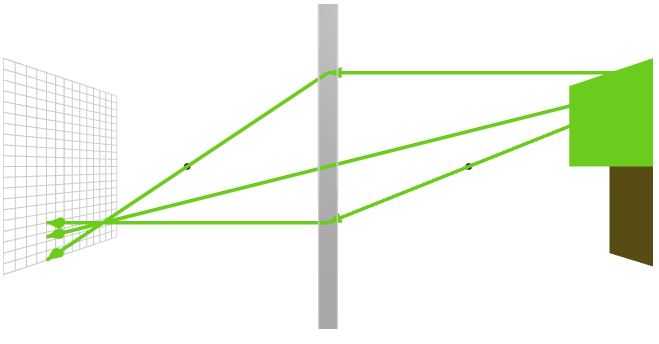
\includegraphics[width=8cm]{images/outoffocus.png}
\end{figure}

Once all slides are  ancreated, they needed to be formatted into a webpage that would be accessible to students or any aspiring photographers. Padding and heights are used to control the spacing of the elements and sections for readability. Animations alone won't do a very good job of explaining what is happening so we supplement each slide with a caption. The captions introduce concepts, define terms, and aid in the development of the explanations. The combination of animations and explanations makes for a potent learning tool. At the end of the webpage we include a link to the interactive camera demo discussed in the previous section.

\section{Technical Challenges}
There were considerable technical challenges that we faced in the creation of
this project which make this project appear deceptively simple. The biggest
challenge faced by our group was having to learn the language and structure of
these new packages. These packages have a unique syntax and learning how to use
them effectively was not a trivial task. Some of the packages, Mathbox2 in
particular, were severely lacking in documentation and the documentation that
did exist was often inadequate to fully explain certain functionalities. One of
the members had also never used JavaScript before, so there was a small
learning curve present at the beginning of the project for him. Through
persistence and by going through examples, we were able to get comfortable
enough with the libraries to create our final result.

\subsection{Camera Demo Challenges}
There were a few minor technical challenges when trying to create the
split-screen view for the interactive camera demo. Creating the split-screen
windows was simple enough; it only required making two different semi-identical
scenes and rendering them with the separate cameras. The difficulty lied when
trying to render the lights and objects in the scenes themselves. For whatever
reason, trying to add an object to more than one scene and rendering that
object in both scenes will not work. Changing the lighting for only one scene
(the main scene remaining well lit) also required creating two separate
instances of the light objects in order to change them separately. We initially
believed that we could just add the objects to both scenes and manipulate them
as children of the scene of interest (i.e. scene1.hemisphereLight). Our
solution was to just create two instances of everything by calling a function
which generates our objects. Each set would be added to a scene and would
render them separately

\subsection{Camera Animation Challenges}
The technical challenges we faced when trying to create the presentations were
numerous. As mentioned before, this was mostly due to having to get accustomed
to learning a brand new library which is unlike anything either of us had used
before and the documentation was a little sparse. We faced organizational
challenges in the sense that we had to decide what functions were important to
create and then trying to implement them and have them work as intended. A
minor bug that was encountered for which we ran out of time to properly solve,
is that when the user advances the slides using the arrow keys on their
keyboard, both slide presentations will advance. This is mildly inconvenient
for a person trying to scroll down after finishing the first section and begin
learning the second set of material. Our solution was to create a "reset"
functionality. When the user presses the spacebar key, the slides reset to the
beginning. This works rather well as a fix.

\section{Results and Discussion}
The end result of our project is a website
(\url{http://samlau.me/camera-interact}) where people who want to learn
about how cameras work can go and use. It begins by going through a bit of
camera backstory and then promptly introduces the user to the animations. The
user goes and clicks back and forth until they understand the concepts and then
they click and go on to interact with our small demo. Provided below are two
pictures of adjacent slides that try to explain ray tracing. Figs. 4(a) and
4(b) show the beginning of the ray tracing explanation: how the horizontal
principal ray is bent through the focal point to the image location. We're
quite pleased with the way the animations ended up. They are pleasing to look
at, the user can rotate the scene and look at it from different angles, and we
believe the explanations paired with the slides make for an effective learning
tool. After the section on depth of field effects, the user will scroll down a
bit and click on a link to our camera demo
(\url{http://samlau.me/camera-interact/full_camera_demo.html}). Two
screenshots comparing two different camera settings are provided below in Figs.
5(a) and 5(b).

We believe we have created an effective learning tool for people who want to
know how cameras work. This not the first attempt that has been made to create
a tool such as this one. There is a DSLR camera simulator \cite{camerasim} that
simulates environments and can simulate photographs taken with different
settings (the scenes are computer generated), however, it costs money. A person
with only a passing curiosity or a  student may not want to invest in these
tools. There are free tools \cite{cannonsim, interactiveap} that use actual
camera settings and either real photographs or digital manipulations of images
to simulate photographs but they lack the background information and theory as
to why it's the case. They also only focus on a few aspects such as exposure or
aperture settings. Our tool provides an intuition about cameras and camera
settings and gives the user an important theoretical background that they can
then use to begin to experiment with cameras. We believe that a particularly
effective way to learn would be to use our project and then supplement it with
free software so that the user understands why settings do what they do.

\begin{figure}[h]%
    \centering
    \subfloat[Ray diagram step 1]{{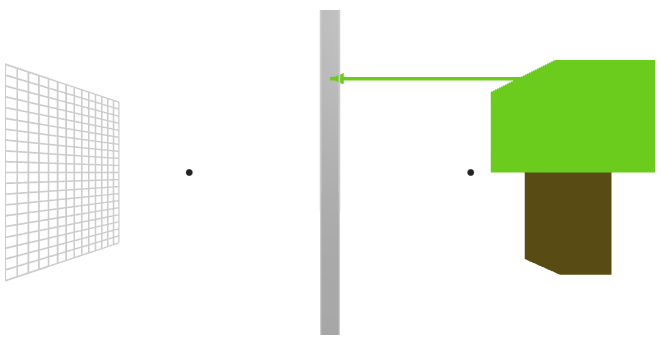
\includegraphics[width=3cm]{images/step1.png} }}%
    \qquad
    \subfloat[Ray diagram step 2]{{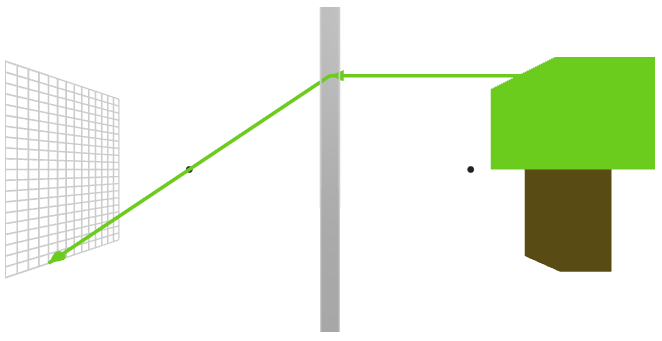
\includegraphics[width=3cm]{images/step2.png} }}%
    \caption{Animations in the presentation}%
    \label{fig:example}%
    \qquad
    \subfloat[Lower shutter speed]{{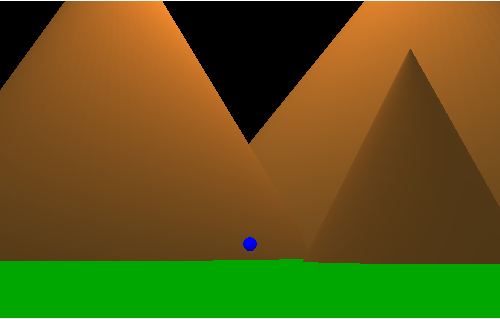
\includegraphics[width=3.3cm]{images/darker.png} }}%
    \qquad
    \subfloat[Higher shutter speed]{{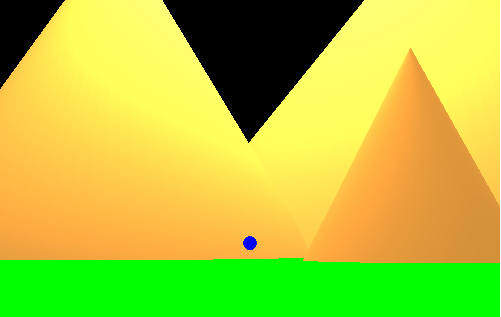
\includegraphics[width=3.3cm]{images/lighter.png} }}%
    \caption{Lighting changes in the demo}%
    \label{fig:example}%
\end{figure}

\bigskip
\bigskip
\bigskip

\section{Member Contributions}

Jeronimo contributed the following:

\begin{enumerate}
  \item Scene objects and scene lights
  \item Camera controls and rendering static image
  \item FOV and aperture change for camera demo
  \item GUI for camera demo
  \item Basic lighting model
  \item Animations for lenses, aperture, and circle of confusion
\end{enumerate}

Sam contributed the following:

\begin{enumerate}
  \item Project idea and storyboarding
  \item Library selection
  \item Skeleton to render scene and slides
  \item Reusable functions to render pixel grid, tree, and light rays
  \item Animations for sensor, pinhole camera, and field of view
  \item Final HTML page and controls for slide text
\end{enumerate}

\section{Project Video Link}

Link to project video: \url{https://youtu.be/GtvFududmN8}

\bibliographystyle{unsrt}
\bibliography{references}


%\balancecolumns
\end{document}
